% Propósito: mostrar cómo magnitudes derivadas se construyen combinando
% dimensiones de masa [M], longitud [L] y tiempo [T].
% Origen: v=d/Delta t, a=Delta v/Delta t, F=ma, p=F/A,
% rho=m/V y f=N/Delta t, con N adimensional.
% Descripción accesible: cuatro cadenas muestran que longitud dividida por
% tiempo produce rapidez y, al dividir otra vez por tiempo, aceleración; masa
% por aceleración produce fuerza y fuerza dividida por área produce presión;
% masa dividida por volumen produce densidad; uno dividido por tiempo produce
% frecuencia.
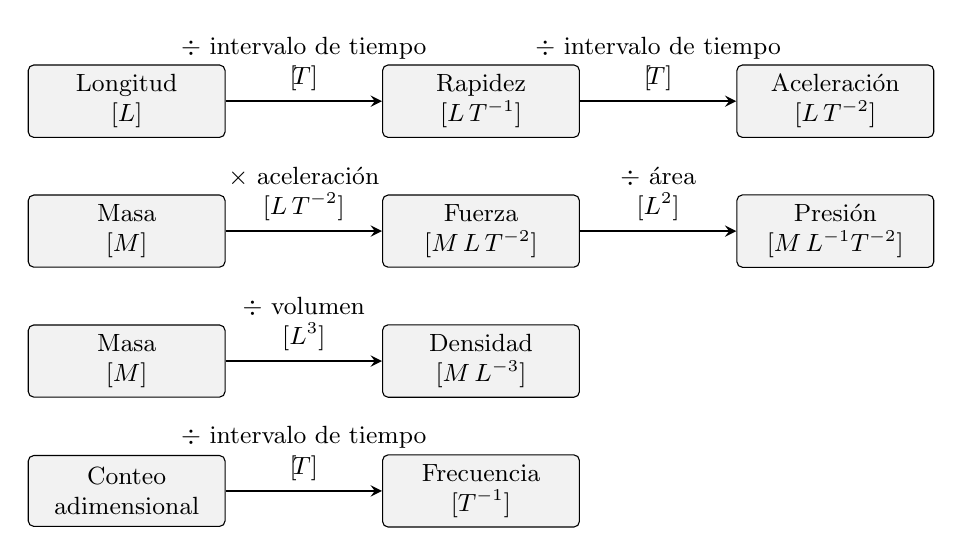
\begin{tikzpicture}[
    font=\small,
    >=stealth,
    magnitud/.style={
        draw,
        rounded corners=2pt,
        minimum width=2.5cm,
        minimum height=0.9cm,
        align=center,
        fill=black!5
    }
]
    \node[magnitud] (longitud) at (0,0) {Longitud\\\([L]\)};
    \node[magnitud] (rapidez) at (4.5,0) {Rapidez\\\([L\,T^{-1}]\)};
    \node[magnitud] (aceleracion) at (9,0) {Aceleración\\\([L\,T^{-2}]\)};
    \draw[->,thick] (longitud.east) -- node[above,align=center]
        {\(\div\) intervalo de tiempo\\\([\!T]\)} (rapidez.west);
    \draw[->,thick] (rapidez.east) -- node[above,align=center]
        {\(\div\) intervalo de tiempo\\\([\!T]\)} (aceleracion.west);

    \node[magnitud] (masa-f) at (0,-1.65) {Masa\\\([M]\)};
    \node[magnitud] (fuerza) at (4.5,-1.65) {Fuerza\\\([M\,L\,T^{-2}]\)};
    \node[magnitud] (presion) at (9,-1.65) {Presión\\\([M\,L^{-1}T^{-2}]\)};
    \draw[->,thick] (masa-f.east) -- node[above,align=center]
        {\(\times\) aceleración\\\([L\,T^{-2}]\)} (fuerza.west);
    \draw[->,thick] (fuerza.east) -- node[above,align=center]
        {\(\div\) área\\\([L^{2}]\)} (presion.west);

    \node[magnitud] (masa-rho) at (0,-3.3) {Masa\\\([M]\)};
    \node[magnitud] (densidad) at (4.5,-3.3) {Densidad\\\([M\,L^{-3}]\)};
    \draw[->,thick] (masa-rho.east) -- node[above,align=center]
        {\(\div\) volumen\\\([L^{3}]\)} (densidad.west);

    \node[magnitud] (uno) at (0,-4.95) {Conteo\\adimensional};
    \node[magnitud] (frecuencia) at (4.5,-4.95) {Frecuencia\\\([T^{-1}]\)};
    \draw[->,thick] (uno.east) -- node[above,align=center]
        {\(\div\) intervalo de tiempo\\\([\!T]\)} (frecuencia.west);
\end{tikzpicture}
